\section{Introduction}

Immersive systems are increasingly used for remote operation~\cite{haidegger2011surgery}, simulation-based training~\cite{radianti2020systematic}, and socially interactive environments~\cite{li2021social,wei2022communication}. In these settings, users rarely engage in a single mode of interaction. Instead, they coordinate manual control, spoken communication, and decision making within the same task. Such coordination draws on multiple, partially independent cognitive resources including processing stages, processing codes, perceptual modalities, and response modalities~\cite{wickens2008multiple} that may compete for limited capacity, and is plausibly vulnerable to disruption when users are under acute stress -- a common situational factor in real-world immersive use. Whether stress degrades VR interaction uniformly, or selectively affects components with different resource demands, remains an open question.

Prior work on situationally-induced impairments and disabilities (SIID) has typically studied stress and task performance in non-immersive settings and on isolated tasks~\cite{sears2003computers,sarsenbayeva2019measuring}, without explicitly relating stress effects to the resource profiles of the interaction components involved. Without such a framing, it is difficult to anticipate which aspects of immersive interaction are most likely to break down under stress, or to design adaptive support for the specific component being affected, such as manual selection, speech production, or planning and execution.

To address this, we adopt Multiple Resource Theory (MRT)~\cite{wickens2008multiple} as a task-selection framework. MRT models human performance as depending on multiple partially independent resource channels, providing a principled basis for decomposing complex VR interaction into components with distinct demand profiles (Figure~\ref{fig:mrt}). Guided by MRT, we selected three controlled tasks that recur across immersive systems: a \textit{target acquisition} task~\cite{li2025estimating} for perceptual-motor interaction, a \textit{reading aloud} task~\cite{dillon2021real} for verbal production, and a \textit{Tower of London} task~\cite{shallice1982specific} for executive planning. Rather than directly quantifying resource competition, we use these tasks as an initial empirical step toward understanding how stress modulates behaviour across different resource profiles.

We instantiate this design in a controlled experiment using the Virtual Reality Trier Social Stress Test (VR-TSST)~\cite{liszio2018relaxing}, combining behavioural performance, speech features, and physiological responses. The results do not support a uniform degradation account. In particular, the three interaction components show distinct patterns and magnitudes of change under stress, indicating that situational impairments in VR are task-specific rather than global.

\textbf{Contributions.} (1)~We extend SIID research to immersive VR by examining acute stress across three recurring interaction tasks: target acquisition, reading aloud task, and Tower of London planning, alongside subjective and physiological stress measures. (2)~We introduce an MRT-informed task-probe framing for reasoning about stress-related SIID in complex VR tasks, and provide empirical evidence that acute stress does not uniformly impair VR interaction. (3)~We draw out implications for stress-aware VR systems, arguing that adaptive support should jointly consider the user's stress state and the resource demands of the current task.

% As immersive systems are increasingly used in scenarios such as remote operation~\cite{haidegger2011surgery}, simulation-based training~\cite{radianti2020systematic}, and socially interactive environments~\cite{li2021social,wei2022communication}, users are often required to coordinate multiple forms of interaction within the same setting, including manual control, spoken communication, and decision making. Such complex interaction does not rely on a single cognitive process, but instead requires the coordination of multiple resource channels that may compete for limited capacity. Under stress, this coordination may be further disrupted, potentially leading to uneven or task-specific changes in performance rather than uniform degradation.

\begin{figure*}[!t]
    \centering
    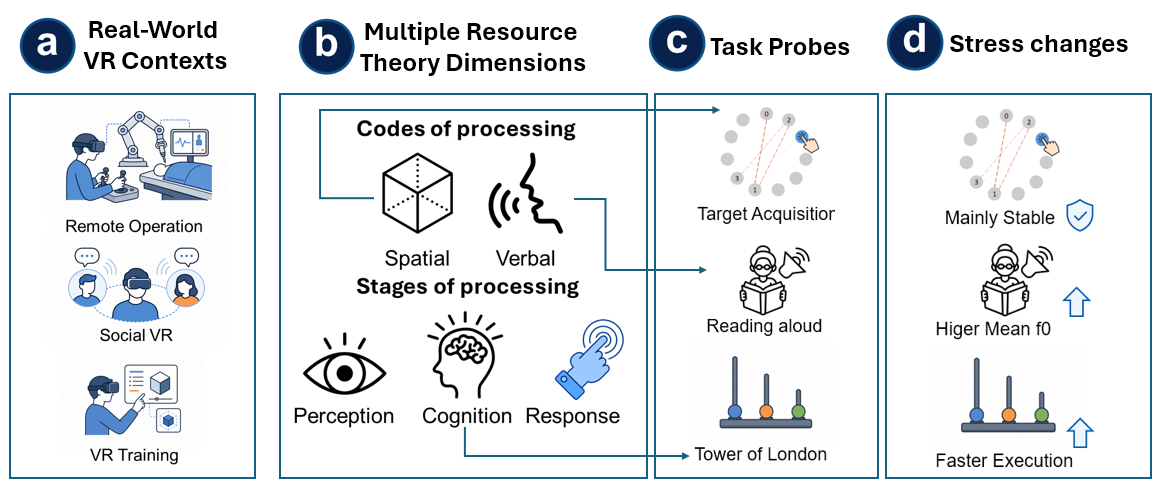
\includegraphics[width=1\textwidth]{Figure/intro.png}
    \caption{Overview of the MRT-informed task-probe approach. We decompose VR interaction demands using selected MRT dimensions and examine stress effects through target acquisition, reading aloud, and Tower of London probes.}
    \label{fig:mrt}
\end{figure*}
